% !TEX root =../LibroTipoETSI.tex
\chapter{Arquitectura de la plataforma}\LABCHAP{ARQ}
\pagestyle{esitscCD}

\section{Diseño de la arquitectura}

Con motivo de no hacer esta
memoria demasiado extensa, se omitirán todas las comparativas que se han hecho
entre diferentes protocolos y servicios y todos los cambios realizados desde la
primera versión hasta la definitiva. De esta forma podremos centrarnos en
describir la arquitectura final.

Desde el primer diseño de la arquitectura hasta el actual se ha pasado por un
enorme proceso de simplificación en el cual se han eliminado bucles, conexiones
redundantes, servicios innecesarios, etc. Se puede decir que la arquitectura
actual consta de los componentes mínimos para llevar a cabo su funcionalidad.

Todas las decisones realizadas para elegir la tecnología más adecuada a la hora
de la implementación del sistema se basan en cinco premisas:

\begin{itemize}\itemsep1pt \parskip0pt \parsep0pt
\item \indexit{Bidireccionalidad:} Los datos debe poder fluir en ambos sentidos. Desde el
dispositivo hasta la lógica del usuario y en sentido contrario.
\item \indexit{Tiempo real:} Los datos deben pasar de un extremo a otro en un tiempo mínimo.
\item \indexit{Persistencia:} El sistema debe ser capaz de almacenar los datos obtenidos para
que puedan ser consultados en cualquier momento. Además debe permitirse el uso
de filtros para obtener la información.
\item \indexit{Monitorización:} El sistema debe ofrecer unas herramientas que ofrezcan
información acerca del estado de sus componentes.
\item \indexit{Tenencia múltiple:} Un despliegue de la plataforma debe permitir ser usada por
varios usuarios u organizaciones.
\end{itemize}

Además, el diseño debe ser lo suficientemente genérico para que cualquier
usuario, independientemente del tipo de datos que quiera enviar, pueda hacer uso
del sistema.

\section{Funcionalidad de la arquitectura}

\subsection{Bidireccionalidad}

La plataforma está diseñada con el objetivo de permitir la comunicación de forma
bidireccional. Como tiene una interfaz con los dispositivos y otra con los
servicios del cliente, tenemos que garantizar que los protocolos que usemos en
ambos casos nos permitan bidireccionalidad.

\subsubsection{Bidireccionalidad en la interfaz con los servicios del cliente}

En el paradigma clásico de internet (HTTP), la comunicación siempre va de
cliente a servidor. El servidor nunca envía ningún dato al cliente, sino que el
cliente debe obtener los datos como respuesta a una petición que él mismo
realice, pero no puede ser notificado en el momento de que haya un nuevo dato.
Esto representa un problema a la hora de conseguir tiempo real.

Una primera solución sería que el cliente constantemente realice peticiones al
servidor para ver si hay datos nuevos para él. Esto es un método poco eficiente
y sólo permite una ``ilusión'' de que obtenemos los datos en tiempo real. Además
este método no es escalable, pues si tenemos miles de clientes sería muy costoso
que estén constantemente haciendo peticiones al servidor ya que cada conexión
supone una reserva y posterior liberación de recursos.

Afortunadamente, en la actualidad existen numerosas alternativas a este método
que permiten la comunicación bidireccional entre cliente y servidor de forma
eficiente. Este paradigma se conoce como comet.

\epigraph{En el desarrollo web, Comet es un neologismo para describir un modelo de
aplicación web en el que una petición HTTP mantenida abierta permite a un
servidor web enviar datos a un navegador por Tecnología Push, sin que el
navegador los solicite explícitamente. Comet es un término paraguas de múltiples
técnicas para conseguir esta interacción.}{Wikipedia}

Hay varias formas de implementar comet, se ha elegido el protocolo STOMP, que
permite a los servicios del cliente establecer una conexión TCP persistente y
recibir datos en tiempo real sin realizar consultas períodicas. La conexión TCP
se mantiene y así se evita estar constantemente reservando y liberando recursos.
El servidor enviará una notificación a través de la conexión TCP establecida.

\subsubsection{Bidireccionalidad en la interfaz con los dispositivos}

En cuanto al extremo contrario, es importante que los dispositivos también sean
capaces de recibir datos en tiempo real desde la plataforma.

Podríamos usar la misma idea que en la otra interfaz, sin embargo, existe un
protocolo muy popular conocido como MQTT que es fácil de implementar en muchos
dispositivos. A diferencia de HTTP, MQTT sí permite una comunicación
bidireccional, por lo que podemos usar dicho protocolo para comunicar también
los dispositivos con la plataforma sin mayor problema.

\subsection{Tiempo real}

El diseño actual de la arquitectura se centra en ofrecer una comunicación
extremo a extremo sin que, en ningún momento, un elemento tenga que solicitar
los datos explícitamente al elemento que le precede, sino que será notificado
por éste cuando haya nuevos datos.

Los datos irán fluyendo por toda la infraestructura hasta llegar al cliente que,
por ejemplo, puede mostrarlo en una web en tiempo real, almacenarlo en una base
de datos o enviar una notificación push a un dispositivo móvil. En ningún
momento el dato se quedará en un elemento intermedio a la espera de que el
siguiente componente lo pida explícitamente.

No debe asumirse que este flujo reactivo impida el agrupamiento de varios
mensajes en uno (batching). Lo que el concepto de flujo reactivo realmente
implica es que el elemento que recibe un dato decide cuando enviarlo al
siguiente, en lugar de esperar que lo soliciten explícitamente.

Como ya se ha indicado antes, la única espera podría ser para realizar batching
y así aumentar la eficiencia del sistema. Una posible mejora sobre la
implementación actual sería hacer agrupaciones de mensajes cuyo tamaño sea
dinámico y dependa de la carga del sistema. Cuando el sistema está saturado, los
mensajes se agrupan en lotes de mensajes de mayor tamaño, mientras que si el
sistema está descargado la granularidad de los mensajes es mayor. Otra opción
sería realizar batching para los clientes gratuitos mientras que para los
clientes de pago se le ofrece granularidad total y, por lo tanto, un tiempo de
respuesta menor.

\subsection{Persistencia}

El usuario puede obtener sus datos de dos formas diferente:

Streaming: Los datos son entregados en tiempo real al cliente y éste debe
procesarlos conforme van llegando. Los filtros debe aplicarlos el usuario.

Query: El cliente puede decidir realizar una consulta a la API cuando él lo
decida para obtener los datos. Pueden establecerse ciertos filtros, por ejemplo,
puede obtener todos los mensajes de un dispositivo en un rango de tiempo.

Obviamente, para el segundo caso es obligatorio que el sistema sea capaz de
persistir los datos. Por ello el sistema dispondrá de diferentes bases de datos
para poder llevar a cabo esta tarea.

\subsection{Monitorización}

El cliente en cualquier momento debe saber en qué estado se encuentra la
plataforma, para ello primero tendremos que analizar el sistema continuamente y
exponer al cliente los datos que puedan ser de su interés.

Para ello se hará uso de tecnología como ELK, Prometheus, Consul y otras que
obtendrán métricas de uso del sistema: recursos usados y otros parámetros que
puedan ser relevantes para conocer el funcionamiento del sistema. De todos estos
datos obtenidos, podemos exponer a los clientes los que puedan ser más
interesantes para ellos, como por ejemplo, el volumen de datos persistidos o el
tráfico cursado ya que pueden ser usados par la tarificación del servicio.

\subsection{Tenencia múltiple}

La plataforma debe permitir el uso por múltiples organizaciones o usuarios.
Cada usuario puede tener una o varias flotas de dispositivos que sean
independientes de los otros usuarios. Aunque los datos pasen por la misma
plataforma debe existir un aislamiento que impida a un usuario obtener datos de
otro.

Otra ventaja de la tenencia múltiple es que una organización puede realizar un
despliegue de la plataforma y ofrecer los servicios a otras organizaciones.

\section{Estructura}

\begin{figure}[htbp]
\centering
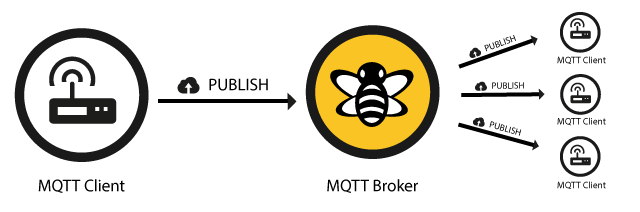
\includegraphics[width=\linewidth]{contenido/figuras/fig001}
\caption{Estructura de un aplicación que use la plataforma}
\label{fig:figura1}
\end{figure}

Como vemos en la \FIG{figura1}, la plataforma se sitúa como elemento intermedio entre
los dispositivos y la lógica del usuario. El objetivo es ofrecer de forma
transparente y eficiente un canal de comunicación al usuario para que éste pueda
centrarse en su negocio, que es ofrecer una serie de servicios al usuario final
sin tener que preocuparse por cómo se mueven los datos.

Puesto que la plataforma soporta multi tennant, múltiples usuario pueden
compartir la plataforma o una organización puede encargarse de mantenerla y
ofrecer sus servicios a los usuarios finales.

Sabiendo todo esto, podríamos definir la plataforma de la siguiente manera:

Es una plataforma que permite a los desarrolladores de dispositivos inteligentes
comunicar sus dispositivos con su lógica de negocio de forma transparente,
rápida, fiable y segura.
Para usar la plataforma habrá que preparar a los dispositivos que se distribuyan
para que se comuniquen con la API y por otro lado habrá que diseñar los
servicios para que obtengan los datos también de la API.

A continuación se puede ver un esquema de la arquitectura final en \FIG{figura2}.

\begin{figure}[htbp]
\centering
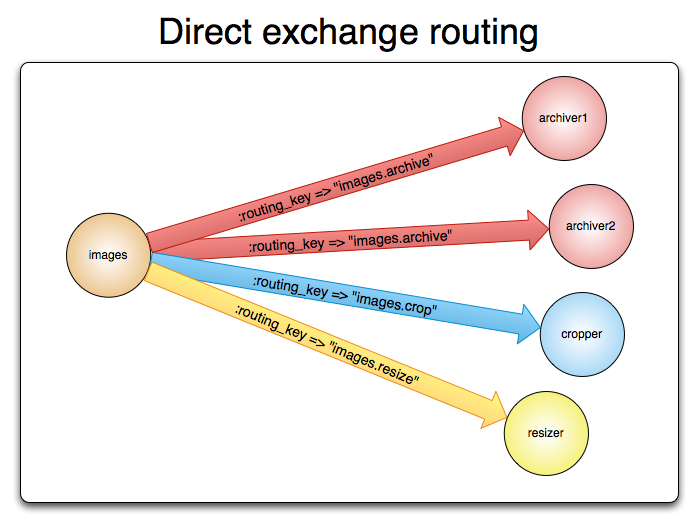
\includegraphics[width=0.6\linewidth]{contenido/figuras/fig002}
\caption{Estructura interna de la plataforma}
\label{fig:figura2}
\end{figure}

\section{Elementos}

En la figura se pueden ver los elementos de la plataforma, situados entre los
dispositivos y la lógica de negocio del usuario. Tenemos los siguientes
componentes:

\subsection{Elementos finales}

Dispositivos: Los dispositivos son los elementos que se pretenden comunicar con
la lógica del usuario. Un dispositivo puede ser cualquier cosa que envíe o
reciba datos. Pueden desempeñar el rol de sensor, actuador o ambos. Están
totalmente fuera del ámbito de la plataforma, es responsabilidad del usuario su
desarrollo y mantenimiento.

Módulos: Una alternativa para poder conectar dispositivos a la plataforma es
usar módulos o dispositivos virtuales. En este caso se crearía una aplicación
que se comunica directamente con la plataforma y simula ser un dispositivo.
Hace de puente entre los dispositivos reales, de forma que se pueden simplificar
los dispositivos. Es útil para adaptar a la plataforma dispositivos existentes.

\subsection{Elementos de la plataforma}

API: Es el componente que permite a los usuarios comunicarse con la plataforma.
Tanto los dispositivos como los servicios propios del usuario usarán la API. Es
tarea de la API el registro de los dispositivos, el registro de usuarios y otras
tareas de gestión así como permite hacer consultas para obtener datos
almacenados en la plataforma.

Sistema de mensajes: Es el componente central de la arquitectura. Por él pasan
los mensajes enviados por los otros elementos. Permite balanceo de carga entre
múltiples instancias, persistencia, sincronización, etc.

Bases de datos: La persistencia del sistema. Múltiples bases de datos se
encargan de almacenar los datos recibidos que deben ser persistidos. También
será necesaria almacenar información de usarios y dispositivos registrados.

Procesador de flujos: Este componente obtiene los datos en crudo de la cola de
mensajes, los trata y los almacena en la bases de datos. Puede ser interesante
añadir algunos metadatos a la información recibida antes de almacenarse.

Monitorización: Son los servicios encargados de obtener información sobre el
consumo y el estado de los elementos en del sistema. Detectará caídas de
componentes y posibles cuellos de botella.

\subsection{Elementos del usuario}

Lógica de cliente: El cometido de la plataforma es ofrecer un servicio a esta
lógica para que pueda comunicarse con los elementos finales. Se comunicará con
la API y el sistema de colas para obtener y enviar datos.
